
%(BEGIN_QUESTION)
% Copyright 2009, Tony R. Kuphaldt, released under the Creative Commons Attribution License (v 1.0)
% This means you may do almost anything with this work of mine, so long as you give me proper credit

In this process, maple syrup is heated as it passes through a steam heat exchanger, then enters an evaporator where the water boils off.  The purpose of this is to raise the sugar concentration of the syrup, making it suitable for use as a food topping.  A level control system (LT, LIC, and LV) maintains constant syrup level inside the evaporator, while an analytical control system (AT, AIR, AC, and AV) monitors the sugar concentration of the syrup and adjusts steam flow to the heat exchanger accordingly.

$$\includegraphics[width=15.5cm]{i02937x01.eps}$$

Suppose the steam tubes inside the heat exchanger become coated with residue from the raw maple syrup, making it more difficult for heat to transfer from the steam to the syrup.  This makes the heat exchanger less efficient, which will undoubtedly affect the process.

\vskip 10pt

Describe in detail the effect this heat exchanger problem will have on the performance of the analytical control system.

\vskip 20pt \vbox{\hrule \hbox{\strut \vrule{} {\bf Suggestions for Socratic discussion} \vrule} \hrule}

\begin{itemize}
\item{} Suppose the operations personnel of this maple syrup processing facility wished to have an {\it automatic} method for detecting heat exchanger fouling.  What variable(s) could be measured in this process to indicate a fouled heat exchanger?
\item{} What economic effect will this fouling have on the process?  In other words, does the process become more or less profitable as a result of the heat exchanger fouling?
\end{itemize}

\underbar{file i02937}
%(END_QUESTION)





%(BEGIN_ANSWER)

The analytical control system should still be able to maintain sugar concentration at setpoint, unless the heat exchanger fouling is so extreme that even a wide-open steam valve does not heat the incoming syrup enough to sufficiently concentrate it.

\vskip 10pt

Follow-up question: suppose the heat exchanger fouling really is this bad, but we cannot fix the heat exchanger with the tools we have available.  What would you recommend the operator do to make this system produce on-spec syrup?

%(END_ANSWER)





%(BEGIN_NOTES)

The operator could reduce the incoming feed rate to allow the fouled heat exchanger to sufficiently heat the incoming syrup.

\vskip 20pt \vbox{\hrule \hbox{\strut \vrule{} {\bf Virtual Troubleshooting} \vrule} \hrule}

This question is a good candidate for a ``Virtual Troubleshooting'' exercise.  Presenting the diagram to students, you first imagine in your own mind a particular fault in the system.  Then, you present one or more symptoms of that fault (something noticeable by an operator or other user of the system).  Students then propose various diagnostic tests to perform on this system to identify the nature and location of the fault, as though they were technicians trying to troubleshoot the problem.  Your job is to tell them what the result(s) would be for each of the proposed diagnostic tests, documenting those results where all the students can see.

During and after the exercise, it is good to ask students follow-up questions such as:

\begin{itemize}
\item{} What does the result of the last diagnostic test tell you about the fault?
\item{} Suppose the results of the last diagnostic test were different.  What then would that result tell you about the fault?
\item{} Is the last diagnostic test the best one we could do?
\item{} What would be the ideal order of tests, to diagnose the problem in as few steps as possible?
\end{itemize}

%INDEX% Basics, control loop troubleshooting: determining effect of specified fault(s)
%INDEX% Process: maple syrup concentration (single-effect evaporator)

%(END_NOTES)


